% Diagram of Android activity life cycle
% Author: Pavel Seda 
\documentclass[border=10pt]{standalone}
\usepackage{tikz}
\usetikzlibrary{arrows.meta}
\tikzset{%
  >={Latex[width=2mm,length=2mm]},
  % Specifications for style of nodes:
            base/.style = {rectangle, rounded corners, draw=black,
                           minimum width=4cm, minimum height=1cm,
                           text centered, font=\sffamily},
  activityStarts/.style = {base, fill=blue!30},
       startstop/.style = {base, fill=red!30},
    activityRuns/.style = {base, fill=green!30},
         process/.style = {base, minimum width=2.5cm, fill=orange!15,
                           font=\ttfamily},
}
\begin{document}
% Drawing part, node distance is 1.5 cm and every node
% is prefilled with white background
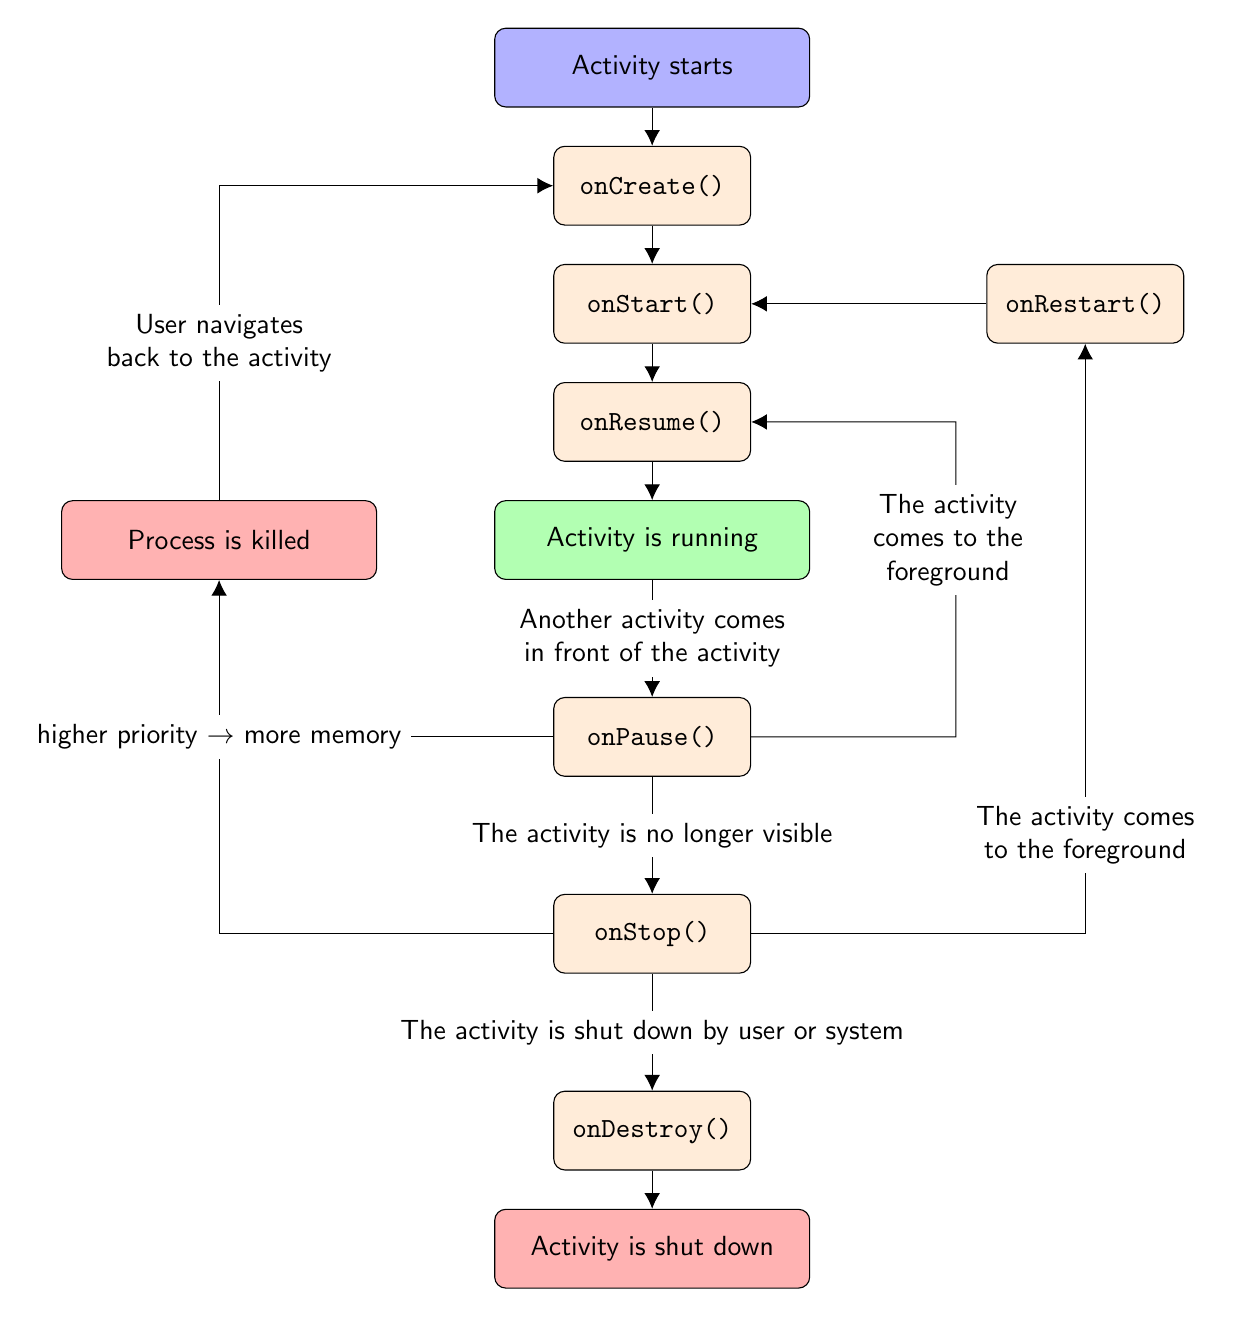
\begin{tikzpicture}[node distance=1.5cm,
		every node/.style={fill=white, font=\sffamily}, align=center]
	% Specification of nodes (position, etc.)
	\node (start)             [activityStarts]              {Activity starts};
	\node (onCreateBlock)     [process, below of=start]          {onCreate()};
	\node (onStartBlock)      [process, below of=onCreateBlock]   {onStart()};
	\node (onResumeBlock)     [process, below of=onStartBlock]   {onResume()};
	\node (activityRuns)      [activityRuns, below of=onResumeBlock]
	{Activity is running};
	\node (onPauseBlock)      [process, below of=activityRuns, yshift=-1cm]
	{onPause()};
	\node (onStopBlock)       [process, below of=onPauseBlock, yshift=-1cm]
	{onStop()};
	\node (onDestroyBlock)    [process, below of=onStopBlock, yshift=-1cm]
	{onDestroy()};
	\node (onRestartBlock)    [process, right of=onStartBlock, xshift=4cm]
	{onRestart()};
	\node (ActivityEnds)      [startstop, left of=activityRuns, xshift=-4cm]
	{Process is killed};
	\node (ActivityDestroyed) [startstop, below of=onDestroyBlock]
	{Activity is shut down};
	% Specification of lines between nodes specified above
	% with aditional nodes for description 
	\draw[->]             (start) -- (onCreateBlock);
	\draw[->]     (onCreateBlock) -- (onStartBlock);
	\draw[->]      (onStartBlock) -- (onResumeBlock);
	\draw[->]     (onResumeBlock) -- (activityRuns);
	\draw[->]      (activityRuns) -- node[text width=4cm]
	{Another activity comes in
		front of the activity} (onPauseBlock);
	\draw[->]      (onPauseBlock) -- node {The activity is no longer visible}
	(onStopBlock);
	\draw[->]       (onStopBlock) -- node {The activity is shut down by
		user or system} (onDestroyBlock);
	\draw[->]    (onRestartBlock) -- (onStartBlock);
	\draw[->]       (onStopBlock) -| node[yshift=1.25cm, text width=3cm]
		{The activity comes to the foreground}
	(onRestartBlock);
	\draw[->]    (onDestroyBlock) -- (ActivityDestroyed);
	\draw[->]      (onPauseBlock) -| node(priorityXMemory)
	{higher priority $\rightarrow$ more memory}
	(ActivityEnds);
	\draw           (onStopBlock) -| (priorityXMemory);
	\draw[->]     (ActivityEnds)  |- node [yshift=-2cm, text width=3.1cm]
		{User navigates back to the activity}
	(onCreateBlock);
	\draw[->] (onPauseBlock.east) -- ++(2.6,0) -- ++(0,2) -- ++(0,2) --
	node[xshift=1.2cm,yshift=-1.5cm, text width=2.5cm]
	{The activity comes to the foreground}(onResumeBlock.east);
\end{tikzpicture}
\end{document}
